\subsection{Overview}

\begin{figure}
  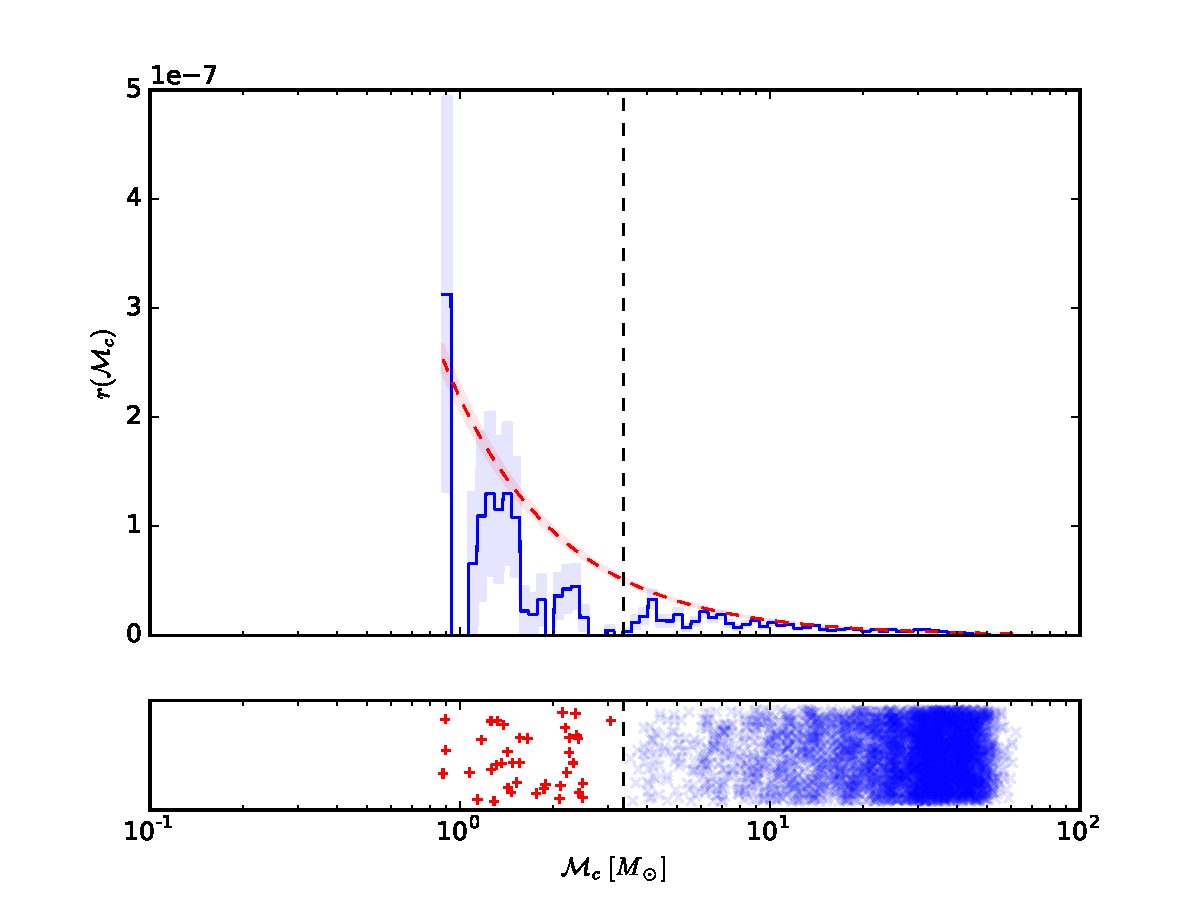
\includegraphics[width=\columnwidth]{img/chirp-mass-distribution}
  \caption{}
  \label{fig:chirp}
\end{figure}

\begin{figure}
  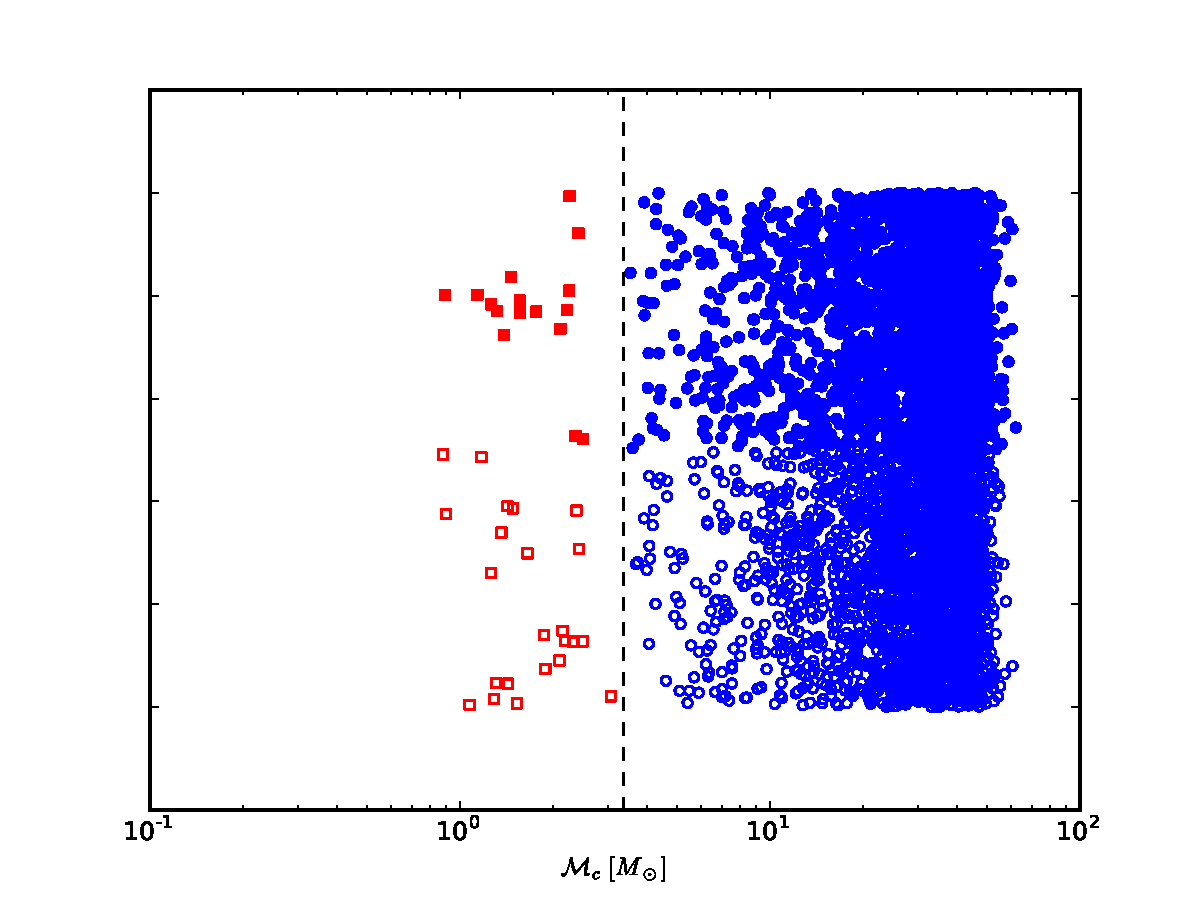
\includegraphics[width=\columnwidth]{img/classifier_comparison}
  \caption{This shows a selected set of the data. The red points represent the events with electromagnetic counterparts, and the blue points represent the events without electromagnetic counterparts. The filled points represent represent the train dataset, and the open points represent the rest of the data. The vertical line indicates the division between the two groups indicated by the classifier.}
  \label{fig:class}
\end{figure}

The GW observatory, the Laser Interferometer Gravitational Wave Observatory (LIGO), can provide very rapid mass estimates of candidate GW events. Since most of these detections are mostly binary black holes and electromagnetic followup is extremely expensive, only a few events can be followed up. We have therefore trained a classifier to determine if an event will have a electromagnetic followup. We trained this classifier on the first half of the data; we simply took the mid-way point betweewn the maximum chirp mass for the electromagnetic counterpart group and the nonelectromagnetic counterpart group. This can be seen in Figure \ref{fig:class}

\subsection{Method}
The classifier was constructed simply by taking the minimum chirp mass event of the other group (no electromagnetic counterparts) and the maximum chirp mass event of the electromagnetic counterpart group and finding the distance between those two events. This trained for the first half of the dataset. The result can be seen in Figure \ref{fig:half}; the vertical line represents half the distance between the maximum chirp mass of the electromagnetic counterpart group and the other group.

\subsection{Results}
The classifier correctly classified the two groups without any contamination. More importantly this was also the case when classifying the full data set. As you can see in Figure \ref{fig:all}, the classifier correctly classified the two groups without any contamination. In the Table \ref{tab:chirp} You can see the chirp mass for the maximum electromagnetic counterpart event and the minimum of the other group along with the chirp mass of the line that divides the group. This shows a clear distinction between the two group.



Figure \ref{fig:chirp} shows the rate vs the chirp mass with the dividing line from the classifier overplotted. This correlates to the two hump structure in the graph that represents the two groups (electromagnetic counterparts and others). Figure ... shows a similar correlation. The dividing clearly separates the two groups in  m$_{1}$-m$_{2}$ parameter space.